\documentclass[]{book}
\usepackage{lmodern}
\usepackage{amssymb,amsmath}
\usepackage{ifxetex,ifluatex}
\usepackage{fixltx2e} % provides \textsubscript
\ifnum 0\ifxetex 1\fi\ifluatex 1\fi=0 % if pdftex
  \usepackage[T1]{fontenc}
  \usepackage[utf8]{inputenc}
\else % if luatex or xelatex
  \ifxetex
    \usepackage{mathspec}
  \else
    \usepackage{fontspec}
  \fi
  \defaultfontfeatures{Ligatures=TeX,Scale=MatchLowercase}
\fi
% use upquote if available, for straight quotes in verbatim environments
\IfFileExists{upquote.sty}{\usepackage{upquote}}{}
% use microtype if available
\IfFileExists{microtype.sty}{%
\usepackage{microtype}
\UseMicrotypeSet[protrusion]{basicmath} % disable protrusion for tt fonts
}{}
\usepackage[margin=1in]{geometry}
\usepackage{hyperref}
\hypersetup{unicode=true,
            pdftitle={Computing for Big Data (BST-262)},
            pdfauthor={Christine Choirat},
            pdfborder={0 0 0},
            breaklinks=true}
\urlstyle{same}  % don't use monospace font for urls
\usepackage{natbib}
\bibliographystyle{apalike}
\usepackage{color}
\usepackage{fancyvrb}
\newcommand{\VerbBar}{|}
\newcommand{\VERB}{\Verb[commandchars=\\\{\}]}
\DefineVerbatimEnvironment{Highlighting}{Verbatim}{commandchars=\\\{\}}
% Add ',fontsize=\small' for more characters per line
\usepackage{framed}
\definecolor{shadecolor}{RGB}{248,248,248}
\newenvironment{Shaded}{\begin{snugshade}}{\end{snugshade}}
\newcommand{\KeywordTok}[1]{\textcolor[rgb]{0.13,0.29,0.53}{\textbf{{#1}}}}
\newcommand{\DataTypeTok}[1]{\textcolor[rgb]{0.13,0.29,0.53}{{#1}}}
\newcommand{\DecValTok}[1]{\textcolor[rgb]{0.00,0.00,0.81}{{#1}}}
\newcommand{\BaseNTok}[1]{\textcolor[rgb]{0.00,0.00,0.81}{{#1}}}
\newcommand{\FloatTok}[1]{\textcolor[rgb]{0.00,0.00,0.81}{{#1}}}
\newcommand{\ConstantTok}[1]{\textcolor[rgb]{0.00,0.00,0.00}{{#1}}}
\newcommand{\CharTok}[1]{\textcolor[rgb]{0.31,0.60,0.02}{{#1}}}
\newcommand{\SpecialCharTok}[1]{\textcolor[rgb]{0.00,0.00,0.00}{{#1}}}
\newcommand{\StringTok}[1]{\textcolor[rgb]{0.31,0.60,0.02}{{#1}}}
\newcommand{\VerbatimStringTok}[1]{\textcolor[rgb]{0.31,0.60,0.02}{{#1}}}
\newcommand{\SpecialStringTok}[1]{\textcolor[rgb]{0.31,0.60,0.02}{{#1}}}
\newcommand{\ImportTok}[1]{{#1}}
\newcommand{\CommentTok}[1]{\textcolor[rgb]{0.56,0.35,0.01}{\textit{{#1}}}}
\newcommand{\DocumentationTok}[1]{\textcolor[rgb]{0.56,0.35,0.01}{\textbf{\textit{{#1}}}}}
\newcommand{\AnnotationTok}[1]{\textcolor[rgb]{0.56,0.35,0.01}{\textbf{\textit{{#1}}}}}
\newcommand{\CommentVarTok}[1]{\textcolor[rgb]{0.56,0.35,0.01}{\textbf{\textit{{#1}}}}}
\newcommand{\OtherTok}[1]{\textcolor[rgb]{0.56,0.35,0.01}{{#1}}}
\newcommand{\FunctionTok}[1]{\textcolor[rgb]{0.00,0.00,0.00}{{#1}}}
\newcommand{\VariableTok}[1]{\textcolor[rgb]{0.00,0.00,0.00}{{#1}}}
\newcommand{\ControlFlowTok}[1]{\textcolor[rgb]{0.13,0.29,0.53}{\textbf{{#1}}}}
\newcommand{\OperatorTok}[1]{\textcolor[rgb]{0.81,0.36,0.00}{\textbf{{#1}}}}
\newcommand{\BuiltInTok}[1]{{#1}}
\newcommand{\ExtensionTok}[1]{{#1}}
\newcommand{\PreprocessorTok}[1]{\textcolor[rgb]{0.56,0.35,0.01}{\textit{{#1}}}}
\newcommand{\AttributeTok}[1]{\textcolor[rgb]{0.77,0.63,0.00}{{#1}}}
\newcommand{\RegionMarkerTok}[1]{{#1}}
\newcommand{\InformationTok}[1]{\textcolor[rgb]{0.56,0.35,0.01}{\textbf{\textit{{#1}}}}}
\newcommand{\WarningTok}[1]{\textcolor[rgb]{0.56,0.35,0.01}{\textbf{\textit{{#1}}}}}
\newcommand{\AlertTok}[1]{\textcolor[rgb]{0.94,0.16,0.16}{{#1}}}
\newcommand{\ErrorTok}[1]{\textcolor[rgb]{0.64,0.00,0.00}{\textbf{{#1}}}}
\newcommand{\NormalTok}[1]{{#1}}
\usepackage{longtable,booktabs}
\usepackage{graphicx,grffile}
\makeatletter
\def\maxwidth{\ifdim\Gin@nat@width>\linewidth\linewidth\else\Gin@nat@width\fi}
\def\maxheight{\ifdim\Gin@nat@height>\textheight\textheight\else\Gin@nat@height\fi}
\makeatother
% Scale images if necessary, so that they will not overflow the page
% margins by default, and it is still possible to overwrite the defaults
% using explicit options in \includegraphics[width, height, ...]{}
\setkeys{Gin}{width=\maxwidth,height=\maxheight,keepaspectratio}
\IfFileExists{parskip.sty}{%
\usepackage{parskip}
}{% else
\setlength{\parindent}{0pt}
\setlength{\parskip}{6pt plus 2pt minus 1pt}
}
\setlength{\emergencystretch}{3em}  % prevent overfull lines
\providecommand{\tightlist}{%
  \setlength{\itemsep}{0pt}\setlength{\parskip}{0pt}}
\setcounter{secnumdepth}{5}
% Redefines (sub)paragraphs to behave more like sections
\ifx\paragraph\undefined\else
\let\oldparagraph\paragraph
\renewcommand{\paragraph}[1]{\oldparagraph{#1}\mbox{}}
\fi
\ifx\subparagraph\undefined\else
\let\oldsubparagraph\subparagraph
\renewcommand{\subparagraph}[1]{\oldsubparagraph{#1}\mbox{}}
\fi

%%% Use protect on footnotes to avoid problems with footnotes in titles
\let\rmarkdownfootnote\footnote%
\def\footnote{\protect\rmarkdownfootnote}

%%% Change title format to be more compact
\usepackage{titling}

% Create subtitle command for use in maketitle
\newcommand{\subtitle}[1]{
  \posttitle{
    \begin{center}\large#1\end{center}
    }
}

\setlength{\droptitle}{-2em}
  \title{Computing for Big Data (BST-262)}
  \pretitle{\vspace{\droptitle}\centering\huge}
  \posttitle{\par}
  \author{Christine Choirat}
  \preauthor{\centering\large\emph}
  \postauthor{\par}
  \predate{\centering\large\emph}
  \postdate{\par}
  \date{2017-08-18}

\usepackage{booktabs}
\usepackage{amsthm}
\makeatletter
\def\thm@space@setup{%
  \thm@preskip=8pt plus 2pt minus 4pt
  \thm@postskip=\thm@preskip
}
\makeatother

\usepackage{amsthm}
\newtheorem{theorem}{Theorem}[chapter]
\newtheorem{lemma}{Lemma}[chapter]
\theoremstyle{definition}
\newtheorem{definition}{Definition}[chapter]
\newtheorem{corollary}{Corollary}[chapter]
\newtheorem{proposition}{Proposition}[chapter]
\theoremstyle{definition}
\newtheorem{example}{Example}[chapter]
\theoremstyle{remark}
\newtheorem*{remark}{Remark}
\begin{document}
\maketitle

{
\setcounter{tocdepth}{1}
\tableofcontents
}
\chapter{Prerequisites}\label{prerequisites}

This is a \emph{sample} book written in \textbf{Markdown}. You can use
anything that Pandoc's Markdown supports, e.g., a math equation
\(a^2 + b^2 = c^2\).

For now, you have to install the development versions of
\textbf{bookdown} from Github:

\begin{Shaded}
\begin{Highlighting}[]
\NormalTok{devtools::}\KeywordTok{install_github}\NormalTok{(}\StringTok{"rstudio/bookdown"}\NormalTok{)}
\end{Highlighting}
\end{Shaded}

Remember each Rmd file contains one and only one chapter, and a chapter
is defined by the first-level heading \texttt{\#}.

To compile this example to PDF, you need to install XeLaTeX.

\chapter{Introduction}\label{intro}

You can label chapter and section titles using \texttt{\{\#label\}}
after them, e.g., we can reference Chapter \ref{intro}. If you do not
manually label them, there will be automatic labels anyway, e.g.,
Chapter \ref{methods}.

Figures and tables with captions will be placed in \texttt{figure} and
\texttt{table} environments, respectively.

\begin{Shaded}
\begin{Highlighting}[]
\KeywordTok{par}\NormalTok{(}\DataTypeTok{mar =} \KeywordTok{c}\NormalTok{(}\DecValTok{4}\NormalTok{, }\DecValTok{4}\NormalTok{, .}\DecValTok{1}\NormalTok{, .}\DecValTok{1}\NormalTok{))}
\KeywordTok{plot}\NormalTok{(pressure, }\DataTypeTok{type =} \StringTok{'b'}\NormalTok{, }\DataTypeTok{pch =} \DecValTok{19}\NormalTok{)}
\end{Highlighting}
\end{Shaded}

\begin{figure}

{\centering 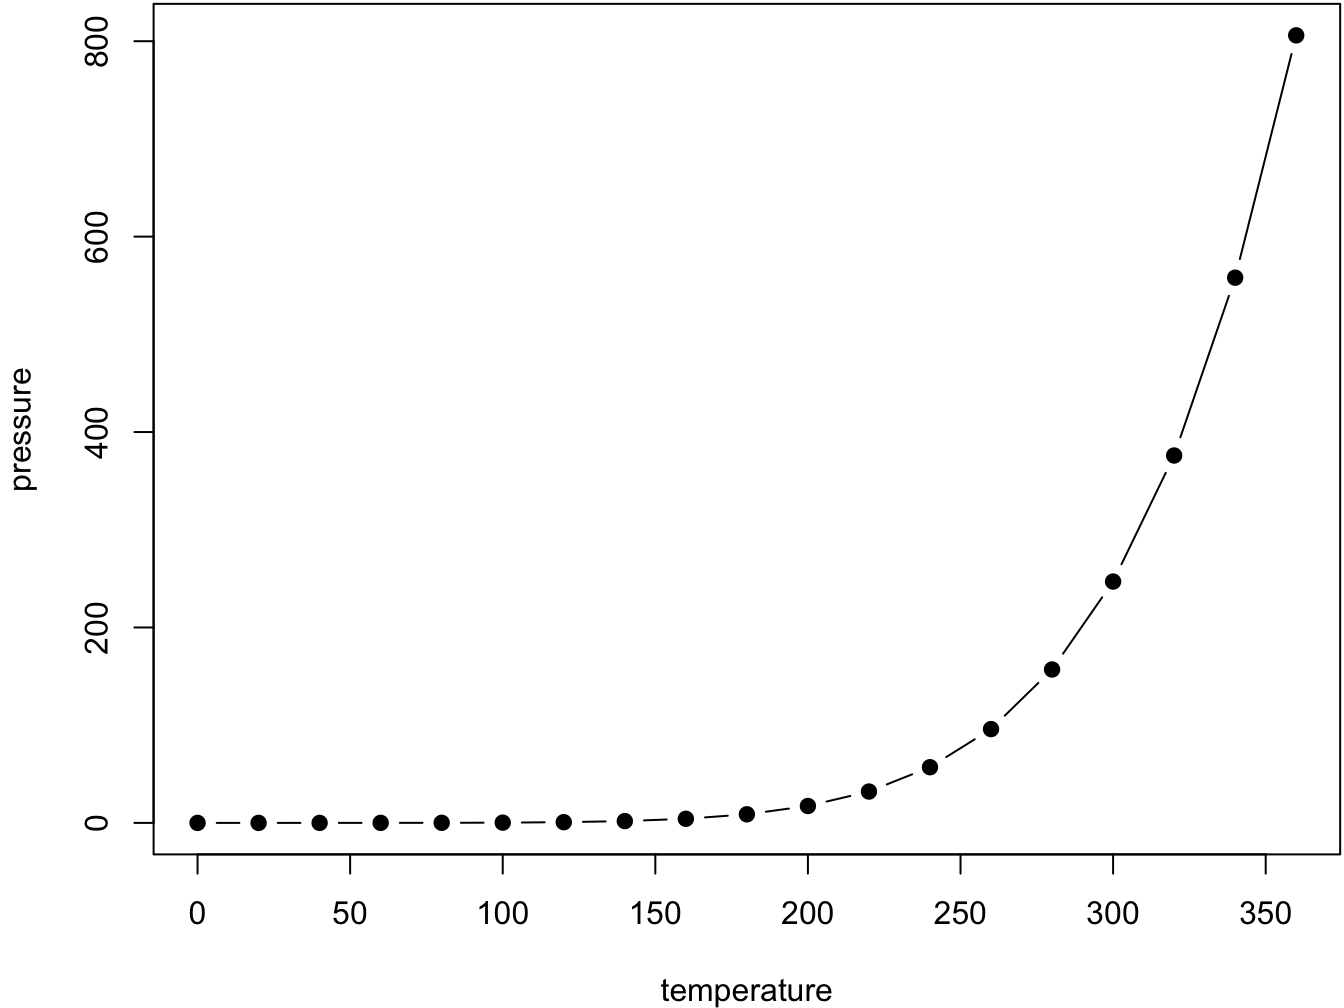
\includegraphics[width=0.8\linewidth]{bookdown-demo_files/figure-latex/nice-fig-1} 

}

\caption{Here is a nice figure!}\label{fig:nice-fig}
\end{figure}

Reference a figure by its code chunk label with the \texttt{fig:}
prefix, e.g., see Figure \ref{fig:nice-fig}. Similarly, you can
reference tables generated from \texttt{knitr::kable()}, e.g., see Table
\ref{tab:nice-tab}.

\begin{Shaded}
\begin{Highlighting}[]
\NormalTok{knitr::}\KeywordTok{kable}\NormalTok{(}
  \KeywordTok{head}\NormalTok{(iris, }\DecValTok{20}\NormalTok{), }\DataTypeTok{caption =} \StringTok{'Here is a nice table!'}\NormalTok{,}
  \DataTypeTok{booktabs =} \OtherTok{TRUE}
\NormalTok{)}
\end{Highlighting}
\end{Shaded}

\begin{table}

\caption{\label{tab:nice-tab}Here is a nice table!}
\centering
\begin{tabular}[t]{rrrrl}
\toprule
Sepal.Length & Sepal.Width & Petal.Length & Petal.Width & Species\\
\midrule
5.1 & 3.5 & 1.4 & 0.2 & setosa\\
4.9 & 3.0 & 1.4 & 0.2 & setosa\\
4.7 & 3.2 & 1.3 & 0.2 & setosa\\
4.6 & 3.1 & 1.5 & 0.2 & setosa\\
5.0 & 3.6 & 1.4 & 0.2 & setosa\\
\addlinespace
5.4 & 3.9 & 1.7 & 0.4 & setosa\\
4.6 & 3.4 & 1.4 & 0.3 & setosa\\
5.0 & 3.4 & 1.5 & 0.2 & setosa\\
4.4 & 2.9 & 1.4 & 0.2 & setosa\\
4.9 & 3.1 & 1.5 & 0.1 & setosa\\
\addlinespace
5.4 & 3.7 & 1.5 & 0.2 & setosa\\
4.8 & 3.4 & 1.6 & 0.2 & setosa\\
4.8 & 3.0 & 1.4 & 0.1 & setosa\\
4.3 & 3.0 & 1.1 & 0.1 & setosa\\
5.8 & 4.0 & 1.2 & 0.2 & setosa\\
\addlinespace
5.7 & 4.4 & 1.5 & 0.4 & setosa\\
5.4 & 3.9 & 1.3 & 0.4 & setosa\\
5.1 & 3.5 & 1.4 & 0.3 & setosa\\
5.7 & 3.8 & 1.7 & 0.3 & setosa\\
5.1 & 3.8 & 1.5 & 0.3 & setosa\\
\bottomrule
\end{tabular}
\end{table}

You can write citations, too. For example, we are using the
\textbf{bookdown} package \citep{R-bookdown} in this sample book, which
was built on top of R Markdown and \textbf{knitr} \citep{xie2015}.

\chapter{Basic tools}\label{basics}

\section{Command line tools}\label{command-line-tools}

\section{Git and GitHub}\label{git-and-github}

\chapter{Packages}\label{packages}

\section{Why?}\label{why}

\begin{itemize}
\item
  Organize your code
\item
  Distribute your code
\item
  Keep versions of your code
\end{itemize}

\section{Structure}\label{structure}

\begin{itemize}
\tightlist
\item
  Folder hierarchy

  \begin{itemize}
  \tightlist
  \item
    \texttt{NAMESPACE}: package import / export
  \item
    \texttt{DESCRIPTION}: metadata
  \item
    \texttt{R/}: R code
  \item
    \texttt{man/}: object documentation (with short examples)
  \item
    \texttt{tests/}
  \item
    \texttt{data/}
  \item
    \texttt{src/}: compiled code
  \item
    \texttt{vignettes/}: manual-like documentation
  \item
    \texttt{inst/}: installed files
  \item
    \texttt{demo/}: longer examples
  \item
    \texttt{exec}, \texttt{po}, \texttt{tools}
  \end{itemize}
\end{itemize}

\section{Building steps}\label{building-steps}

\begin{itemize}
\item
  \texttt{R\ CMD\ build}
\item
  \texttt{R\ CMD\ INSTALL}
\item
  \texttt{R\ CMD\ check}
\end{itemize}

\section{\texorpdfstring{\texttt{R\ CMD\ build}}{R CMD build}}\label{r-cmd-build}

\begin{Shaded}
\begin{Highlighting}[]
\NormalTok{R CMD build --help}
\end{Highlighting}
\end{Shaded}

\emph{Build R packages from package sources in the directories specified
by `pkgdirs'}

\section{\texorpdfstring{\texttt{R\ CMD\ INSTALL}}{R CMD INSTALL}}\label{r-cmd-install}

\begin{Shaded}
\begin{Highlighting}[]
\NormalTok{R CMD INSTALL --help}
\end{Highlighting}
\end{Shaded}

\emph{Install the add-on packages specified by pkgs. The elements of
pkgs can be relative or absolute paths to directories with the package
sources, or to gzipped package `tar' archives. The library tree to
install to can be specified via `--library'. By default, packages are
installed in the library tree rooted at the first directory in
.libPaths() for an R session run in the current environment.}

\section{\texorpdfstring{\texttt{R\ CMD\ check}}{R CMD check}}\label{r-cmd-check}

\begin{Shaded}
\begin{Highlighting}[]
\NormalTok{R CMD check --help}
\end{Highlighting}
\end{Shaded}

\url{http://r-pkgs.had.co.nz/check.html}

\emph{Check R packages from package sources, which can be directories or
package `tar' archives with extension `.tar.gz', `.tar.bz2', `.tar.xz'
or `.tgz'.}

\emph{A variety of diagnostic checks on directory structure, index and
control files are performed. The package is installed into the log
directory and production of the package PDF manual is tested. All
examples and tests provided by the package are tested to see if they run
successfully. By default code in the vignettes is tested, as is
re-building the vignette PDFs.}

\section{\texorpdfstring{Building steps with
\texttt{devtools}}{Building steps with devtools}}\label{building-steps-with-devtools}

\begin{itemize}
\item
  \texttt{devtools::build}
\item
  \texttt{devtools::install}
\item
  \texttt{devtools::check}
\item
  and many others: \texttt{load\_all}, \texttt{document}, \texttt{test},
  \texttt{run\_examples}, \ldots{}
\end{itemize}

\section{Creating an R package}\label{creating-an-r-package}

\subsection{\texorpdfstring{\texttt{utils::package.skeleton}}{utils::package.skeleton}}\label{utilspackage.skeleton}

\begin{Shaded}
\begin{Highlighting}[]
\KeywordTok{package.skeleton}\NormalTok{() }\CommentTok{# "in "fresh" session ("anRpackage")}
\KeywordTok{package.skeleton}\NormalTok{(}\StringTok{"pkgname"}\NormalTok{) }\CommentTok{# in "fresh" session}

\KeywordTok{set.seed}\NormalTok{(}\DecValTok{02138}\NormalTok{)}
\NormalTok{f <-}\StringTok{ }\NormalTok{function(x, y) x+y}
\NormalTok{g <-}\StringTok{ }\NormalTok{function(x, y) x-y}
\NormalTok{d <-}\StringTok{ }\KeywordTok{data.frame}\NormalTok{(}\DataTypeTok{a =} \DecValTok{1}\NormalTok{, }\DataTypeTok{b =} \DecValTok{2}\NormalTok{)}
\NormalTok{e <-}\StringTok{ }\KeywordTok{rnorm}\NormalTok{(}\DecValTok{1000}\NormalTok{)}
\KeywordTok{package.skeleton}\NormalTok{(}\DataTypeTok{list =} \KeywordTok{c}\NormalTok{(}\StringTok{"f"}\NormalTok{,}\StringTok{"g"}\NormalTok{,}\StringTok{"d"}\NormalTok{,}\StringTok{"e"}\NormalTok{), }\DataTypeTok{name =} \StringTok{"pkgname"}\NormalTok{)}
\end{Highlighting}
\end{Shaded}

\subsection{\texorpdfstring{\texttt{devtools::create}}{devtools::create}}\label{devtoolscreate}

\begin{Shaded}
\begin{Highlighting}[]
\NormalTok{devtools::}\KeywordTok{create}\NormalTok{(}\StringTok{"path/to/package/pkgname"}\NormalTok{)}
\end{Highlighting}
\end{Shaded}

\section{Submitting to CRAN}\label{submitting-to-cran}

\url{http://r-pkgs.had.co.nz/release.html}

\section{Using GitHub}\label{using-github}

\url{http://r-pkgs.had.co.nz/git.html}

\section{RStudio and GitHub integration (1 /
7)}\label{rstudio-and-github-integration-1-7}

\section{RStudio and GitHub integration (2 /
7)}\label{rstudio-and-github-integration-2-7}

\section{RStudio and GitHub integration (3 /
7)}\label{rstudio-and-github-integration-3-7}

\section{RStudio and GitHub integration (4 /
7)}\label{rstudio-and-github-integration-4-7}

\section{RStudio and GitHub integration (5 /
7)}\label{rstudio-and-github-integration-5-7}

\section{Command line}\label{command-line}

\begin{Shaded}
\begin{Highlighting}[]
\NormalTok{git init}
\NormalTok{git add *}
\NormalTok{git commit -m }\StringTok{"First commit"}
\NormalTok{git remote add origin git@github.com:harvard-P01/pkgtemplate.git}
\NormalTok{git push -u origin master}
\end{Highlighting}
\end{Shaded}

\section{RStudio and GitHub integration (6 /
7)}\label{rstudio-and-github-integration-6-7}

\section{RStudio and GitHub integration (7 /
7)}\label{rstudio-and-github-integration-7-7}

\section{Installing from GitHub}\label{installing-from-github}

\begin{Shaded}
\begin{Highlighting}[]
\NormalTok{devtools::}\KeywordTok{install_github}\NormalTok{(}\StringTok{"harvard-P01/pkgtemplate"}\NormalTok{)}
\end{Highlighting}
\end{Shaded}

\begin{Shaded}
\begin{Highlighting}[]
\NormalTok{devtools::}\KeywordTok{install_github}\NormalTok{(}\StringTok{"harvard-P01/pkgtemplate"}\NormalTok{,}
                         \DataTypeTok{build_vignettes =} \OtherTok{TRUE}\NormalTok{)}
\end{Highlighting}
\end{Shaded}

\section{\texorpdfstring{\texttt{.gitignore} (RStudio
default)}{.gitignore (RStudio default)}}\label{gitignore-rstudio-default}

\begin{Shaded}
\begin{Highlighting}[]
\NormalTok{.Rproj.user}
\NormalTok{.Rhistory}
\NormalTok{.RData}
\end{Highlighting}
\end{Shaded}

\section{\texorpdfstring{\texttt{.gitignore} (GitHub
default)}{.gitignore (GitHub default)}}\label{gitignore-github-default}

\begin{Shaded}
\begin{Highlighting}[]
\CommentTok{# History files}
\NormalTok{.Rhistory}
\NormalTok{.Rapp.history}

\CommentTok{# Example code in package build process}
\NormalTok{*-Ex.R}

\CommentTok{# RStudio files}
\NormalTok{.Rproj.user/}

\CommentTok{# produced vignettes}
\NormalTok{vignettes/}\ErrorTok{*}\NormalTok{.html}
\NormalTok{vignettes/}\ErrorTok{*}\NormalTok{.pdf}
\end{Highlighting}
\end{Shaded}

\section{RStudio projects}\label{rstudio-projects}

\begin{itemize}
\item
  \texttt{.Rproj} file extension, in our example
  \texttt{pkgtemplate.Rproj}
\item
  A project has its own:

  \begin{itemize}
  \tightlist
  \item
    R session
  \item
    .Rprofile (\emph{e.g.}, to customize startup environment)
  \item
    .Rhistory
  \end{itemize}
\item
  Default working directory is project directory
\item
  Keeps track of project-specific recent files
\end{itemize}

\section{Project options}\label{project-options}

\begin{Shaded}
\begin{Highlighting}[]
\NormalTok{Version:}\StringTok{ }\FloatTok{1.0}

\NormalTok{RestoreWorkspace:}\StringTok{ }\NormalTok{Default}
\NormalTok{SaveWorkspace:}\StringTok{ }\NormalTok{Default}
\NormalTok{AlwaysSaveHistory:}\StringTok{ }\NormalTok{Default}

\NormalTok{EnableCodeIndexing:}\StringTok{ }\NormalTok{Yes}
\NormalTok{UseSpacesForTab:}\StringTok{ }\NormalTok{Yes}
\NormalTok{NumSpacesForTab:}\StringTok{ }\DecValTok{2}
\NormalTok{Encoding:}\StringTok{ }\NormalTok{UTF}\DecValTok{-8}

\NormalTok{RnwWeave:}\StringTok{ }\NormalTok{knitr}
\NormalTok{LaTeX:}\StringTok{ }\NormalTok{pdfLaTeX}

\NormalTok{AutoAppendNewline:}\StringTok{ }\NormalTok{Yes}
\NormalTok{StripTrailingWhitespace:}\StringTok{ }\NormalTok{Yes}

\NormalTok{BuildType:}\StringTok{ }\NormalTok{Package}
\NormalTok{PackageUseDevtools:}\StringTok{ }\NormalTok{Yes}
\NormalTok{PackageInstallArgs:}\StringTok{ }\NormalTok{--no-multiarch --with-keep.source}
\end{Highlighting}
\end{Shaded}

\section{Package documentation}\label{package-documentation}

\begin{itemize}
\item
  Functions and methods
\item
  Vignettes

  \begin{itemize}
  \tightlist
  \item
    PDF
  \item
    \texttt{knitr} (or \texttt{Sweave})
  \end{itemize}
\end{itemize}

\section{Process example}\label{process-example}

Creating R Packages: A Tutorial (Friedrich Leisch, 2009 )

\begin{itemize}
\tightlist
\item
  \url{https://cran.r-project.org/doc/contrib/Leisch-CreatingPackages.pdf}
\end{itemize}

\section{\texorpdfstring{Adding \texttt{linreg.R} in \texttt{R/}
directory}{Adding linreg.R in R/ directory}}\label{adding-linreg.r-in-r-directory}

\begin{Shaded}
\begin{Highlighting}[]
\NormalTok{linmodEst <-}\StringTok{ }\NormalTok{function(x, y) \{}
  \NormalTok{## compute QR-decomposition of x}
  \NormalTok{qx <-}\StringTok{ }\KeywordTok{qr}\NormalTok{(x)}
  \NormalTok{## compute (x’x)^(-1) x’y}
  \NormalTok{coef <-}\StringTok{ }\KeywordTok{solve.qr}\NormalTok{(qx, y)}
  \NormalTok{## degrees of freedom and standard deviation of residuals}
  \NormalTok{df <-}\StringTok{ }\KeywordTok{nrow}\NormalTok{(x) -}\StringTok{ }\KeywordTok{ncol}\NormalTok{(x)}
  \NormalTok{sigma2 <-}\StringTok{ }\KeywordTok{sum}\NormalTok{((y -}\StringTok{ }\NormalTok{x %*%}\StringTok{ }\NormalTok{coef) ^}\StringTok{ }\DecValTok{2}\NormalTok{) /}\StringTok{ }\NormalTok{df}
  \NormalTok{## compute sigma^2 * (x’x)^-1}
  \NormalTok{vcov <-}\StringTok{ }\NormalTok{sigma2 *}\StringTok{ }\KeywordTok{chol2inv}\NormalTok{(qx$qr)}
  \KeywordTok{colnames}\NormalTok{(vcov) <-}\StringTok{ }\KeywordTok{rownames}\NormalTok{(vcov) <-}\StringTok{ }\KeywordTok{colnames}\NormalTok{(x)}
  \KeywordTok{list}\NormalTok{(}
    \DataTypeTok{coefficients =} \NormalTok{coef,}
    \DataTypeTok{vcov =} \NormalTok{vcov,}
    \DataTypeTok{sigma =} \KeywordTok{sqrt}\NormalTok{(sigma2),}
    \DataTypeTok{df =} \NormalTok{df}
  \NormalTok{)}
\NormalTok{\}}
\end{Highlighting}
\end{Shaded}

\section{Running our function}\label{running-our-function}

\begin{Shaded}
\begin{Highlighting}[]
\KeywordTok{data}\NormalTok{(cats, }\DataTypeTok{package =} \StringTok{"MASS"}\NormalTok{)}
\KeywordTok{linmodEst}\NormalTok{(}\KeywordTok{cbind}\NormalTok{(}\DecValTok{1}\NormalTok{, cats$Bwt), cats$Hwt)}
\end{Highlighting}
\end{Shaded}

\begin{verbatim}
## $coefficients
## [1] -0.3566624  4.0340627
## 
## $vcov
##            [,1]        [,2]
## [1,]  0.4792475 -0.17058197
## [2,] -0.1705820  0.06263081
## 
## $sigma
## [1] 1.452373
## 
## $df
## [1] 142
\end{verbatim}

\section{\texorpdfstring{And compare with \texttt{lm} (1 /
2)}{And compare with lm (1 / 2)}}\label{and-compare-with-lm-1-2}

\begin{Shaded}
\begin{Highlighting}[]
\NormalTok{lm1 <-}\StringTok{ }\KeywordTok{lm}\NormalTok{(Hwt ~}\StringTok{ }\NormalTok{Bwt, }\DataTypeTok{data=}\NormalTok{cats)}
\NormalTok{lm1}
\end{Highlighting}
\end{Shaded}

\begin{verbatim}
## 
## Call:
## lm(formula = Hwt ~ Bwt, data = cats)
## 
## Coefficients:
## (Intercept)          Bwt  
##     -0.3567       4.0341
\end{verbatim}

\begin{Shaded}
\begin{Highlighting}[]
\KeywordTok{coef}\NormalTok{(lm1)}
\end{Highlighting}
\end{Shaded}

\begin{verbatim}
## (Intercept)         Bwt 
##  -0.3566624   4.0340627
\end{verbatim}

\section{\texorpdfstring{And compare with \texttt{lm} (2 /
2)}{And compare with lm (2 / 2)}}\label{and-compare-with-lm-2-2}

\begin{Shaded}
\begin{Highlighting}[]
\KeywordTok{vcov}\NormalTok{(lm1)}
\end{Highlighting}
\end{Shaded}

\begin{verbatim}
##             (Intercept)         Bwt
## (Intercept)   0.4792475 -0.17058197
## Bwt          -0.1705820  0.06263081
\end{verbatim}

\begin{Shaded}
\begin{Highlighting}[]
\KeywordTok{summary}\NormalTok{(lm1)$sigma}
\end{Highlighting}
\end{Shaded}

\begin{verbatim}
## [1] 1.452373
\end{verbatim}

\section{Adding ROxygen2
documentation}\label{adding-roxygen2-documentation}

\begin{Shaded}
\begin{Highlighting}[]
\CommentTok{#' Linear regression}
\CommentTok{#'}
\CommentTok{#' Runs an OLS regression not unlike \textbackslash{}code\{\textbackslash{}link\{lm\}\}}
\CommentTok{#'}
\CommentTok{#' @param y response vector (1 x n)}
\CommentTok{#' @param X covariate matrix (p x n) with no intercept}
\CommentTok{#'}
\CommentTok{#' @return A list with 4 elements: coefficients, vcov, sigma, df}
\CommentTok{#'}
\CommentTok{#' @examples}
\CommentTok{#' data(mtcars)}
\CommentTok{#' X <- as.matrix(mtcars[, c("cyl", "disp", "hp")])}
\CommentTok{#' y <- mtcars[, "mpg"]}
\CommentTok{#' linreg(y, X)}
\CommentTok{#'}
\CommentTok{#' @export}
\CommentTok{#'}
\NormalTok{linmodEst <-}\StringTok{ }\NormalTok{function(x, y) \{}
  \NormalTok{## compute QR-decomposition of x}
  \NormalTok{qx <-}\StringTok{ }\KeywordTok{qr}\NormalTok{(x)}
  \NormalTok{## compute (x’x)^(-1) x’y}
  \NormalTok{coef <-}\StringTok{ }\KeywordTok{solve.qr}\NormalTok{(qx, y)}
  \NormalTok{## degrees of freedom and standard deviation of residuals}
  \NormalTok{df <-}\StringTok{ }\KeywordTok{nrow}\NormalTok{(x) -}\StringTok{ }\KeywordTok{ncol}\NormalTok{(x)}
  \NormalTok{sigma2 <-}\StringTok{ }\KeywordTok{sum}\NormalTok{((y -}\StringTok{ }\NormalTok{x %*%}\StringTok{ }\NormalTok{coef) ^}\StringTok{ }\DecValTok{2}\NormalTok{) /}\StringTok{ }\NormalTok{df}
  \NormalTok{## compute sigma^2 * (x’x)^-1}
  \NormalTok{vcov <-}\StringTok{ }\NormalTok{sigma2 *}\StringTok{ }\KeywordTok{chol2inv}\NormalTok{(qx$qr)}
  \KeywordTok{colnames}\NormalTok{(vcov) <-}\StringTok{ }\KeywordTok{rownames}\NormalTok{(vcov) <-}\StringTok{ }\KeywordTok{colnames}\NormalTok{(x)}
  \KeywordTok{list}\NormalTok{(}
    \DataTypeTok{coefficients =} \NormalTok{coef,}
    \DataTypeTok{vcov =} \NormalTok{vcov,}
    \DataTypeTok{sigma =} \KeywordTok{sqrt}\NormalTok{(sigma2),}
    \DataTypeTok{df =} \NormalTok{df}
  \NormalTok{)}
\NormalTok{\}}
\end{Highlighting}
\end{Shaded}

\section{Configure Build Tools}\label{configure-build-tools}

\section{\texorpdfstring{\texttt{man/linmodEst.Rd}}{man/linmodEst.Rd}}\label{manlinmodest.rd}

\begin{Shaded}
\begin{Highlighting}[]
\NormalTok{% Generated by }\KeywordTok{roxygen2} \NormalTok{(}\FloatTok{4.1.1}\NormalTok{):}\StringTok{ }\NormalTok{do not edit by hand}
\NormalTok{% Please edit documentation in R/linmodEst.R}
\NormalTok{\textbackslash{}name\{linmodEst\}}
\NormalTok{\textbackslash{}alias\{linmodEst\}}
\NormalTok{\textbackslash{}title\{Linear regression\}}
\NormalTok{\textbackslash{}usage\{}
\KeywordTok{linmodEst}\NormalTok{(x, y)}
\NormalTok{\}}
\NormalTok{\textbackslash{}arguments\{}
\NormalTok{\textbackslash{}item\{y\}\{response }\KeywordTok{vector} \NormalTok{(}\DecValTok{1} \NormalTok{x n)\}}

\NormalTok{\textbackslash{}item\{X\}\{covariate }\KeywordTok{matrix} \NormalTok{(p x n) with no intercept\}}
\NormalTok{\}}
\NormalTok{\textbackslash{}value\{}
\NormalTok{A list with }\DecValTok{4} \NormalTok{elements:}\StringTok{ }\NormalTok{coefficients, vcov, sigma, df}
\NormalTok{\}}
\NormalTok{\textbackslash{}description\{}
\NormalTok{Runs an OLS regression not unlike \textbackslash{}code\{\textbackslash{}link\{lm\}\}}
\NormalTok{\}}
\NormalTok{\textbackslash{}examples\{}
\KeywordTok{data}\NormalTok{(mtcars)}
\NormalTok{X <-}\StringTok{ }\KeywordTok{as.matrix}\NormalTok{(mtcars[, }\KeywordTok{c}\NormalTok{(}\StringTok{"cyl"}\NormalTok{, }\StringTok{"disp"}\NormalTok{, }\StringTok{"hp"}\NormalTok{)])}
\NormalTok{y <-}\StringTok{ }\NormalTok{mtcars[, }\StringTok{"mpg"}\NormalTok{]}
\KeywordTok{linmodEst}\NormalTok{(y, X)}
\NormalTok{\}}
\end{Highlighting}
\end{Shaded}

\section{Formatted output}\label{formatted-output}

\section{\texorpdfstring{\texttt{DESCRIPTION}}{DESCRIPTION}}\label{description}

\begin{Shaded}
\begin{Highlighting}[]
\NormalTok{Package:}\StringTok{ }\NormalTok{pkgtemplate}
\NormalTok{Type:}\StringTok{ }\NormalTok{Package}
\NormalTok{Title:}\StringTok{ }\NormalTok{What the Package }\KeywordTok{Does} \NormalTok{(Title Case)}
\NormalTok{Version:}\StringTok{ }\FloatTok{0.1}
\NormalTok{Date:}\StringTok{ }\DecValTok{2015-10-24}
\NormalTok{Author:}\StringTok{ }\NormalTok{Who wrote it}
\NormalTok{Maintainer:}\StringTok{ }\NormalTok{Who to complain to <yourfault@somewhere.net>}
\NormalTok{Description:}\StringTok{ }\NormalTok{More about what it }\KeywordTok{does} \NormalTok{(maybe more than one line)}
\NormalTok{License:}\StringTok{ }\NormalTok{What license is it under?}
\NormalTok{LazyData:}\StringTok{ }\OtherTok{TRUE}
\end{Highlighting}
\end{Shaded}

\section{\texorpdfstring{\texttt{NAMESPACE}}{NAMESPACE}}\label{namespace}

\texttt{export}'s automatically generated when parsing ROxygens2
snippets

\begin{Shaded}
\begin{Highlighting}[]
\KeywordTok{export}\NormalTok{(linmodEst)}
\end{Highlighting}
\end{Shaded}

\section{S3 basics}\label{s3-basics}

\begin{Shaded}
\begin{Highlighting}[]
\NormalTok{hello <-}\StringTok{ }\NormalTok{function() \{}
 \NormalTok{s <-}\StringTok{ "Hello World!"}
 \KeywordTok{class}\NormalTok{(s) <-}\StringTok{ "hi"}
 \KeywordTok{return}\NormalTok{(s)}
\NormalTok{\}}

\KeywordTok{hello}\NormalTok{()}
\end{Highlighting}
\end{Shaded}

\begin{verbatim}
## [1] "Hello World!"
## attr(,"class")
## [1] "hi"
\end{verbatim}

\section{S3 basics}\label{s3-basics-1}

\begin{Shaded}
\begin{Highlighting}[]
\NormalTok{print.hi <-}\StringTok{ }\NormalTok{function(...) \{}
  \KeywordTok{print}\NormalTok{(}\StringTok{"Surprise!"}\NormalTok{)}
\NormalTok{\}}

\KeywordTok{hello}\NormalTok{()}
\end{Highlighting}
\end{Shaded}

\begin{verbatim}
## [1] "Surprise!"
\end{verbatim}

\section{S3 and S4 generics}\label{s3-and-s4-generics}

\begin{Shaded}
\begin{Highlighting}[]
\NormalTok{linmod <-}\StringTok{ }\NormalTok{function(x, ...)}
  \KeywordTok{UseMethod}\NormalTok{(}\StringTok{"linmod"}\NormalTok{)}
\end{Highlighting}
\end{Shaded}

\begin{Shaded}
\begin{Highlighting}[]
\NormalTok{linmod.default <-}\StringTok{ }\NormalTok{function(x, y, ...) \{}
  \NormalTok{x <-}\StringTok{ }\KeywordTok{as.matrix}\NormalTok{(x)}
  \NormalTok{y <-}\StringTok{ }\KeywordTok{as.numeric}\NormalTok{(y)}
  \NormalTok{est <-}\StringTok{ }\KeywordTok{linmodEst}\NormalTok{(x, y)}
  \NormalTok{est$fitted.values <-}\StringTok{ }\KeywordTok{as.vector}\NormalTok{(x %*%}\StringTok{ }\NormalTok{est$coefficients)}
  \NormalTok{est$residuals <-}\StringTok{ }\NormalTok{y -}\StringTok{ }\NormalTok{est$fitted.values}
  \NormalTok{est$call <-}\StringTok{ }\KeywordTok{match.call}\NormalTok{()}
  \KeywordTok{class}\NormalTok{(est) <-}\StringTok{ "linmod"}
  \KeywordTok{return}\NormalTok{(est)}
\NormalTok{\}}
\end{Highlighting}
\end{Shaded}

\section{\texorpdfstring{\texttt{print}}{print}}\label{print}

\begin{Shaded}
\begin{Highlighting}[]
\NormalTok{print.linmod <-}\StringTok{ }\NormalTok{function(x, ...) \{}
  \KeywordTok{cat}\NormalTok{(}\StringTok{"Call:}\CharTok{\textbackslash{}n}\StringTok{"}\NormalTok{)}
  \KeywordTok{print}\NormalTok{(x$call)}
  \KeywordTok{cat}\NormalTok{(}\StringTok{"}\CharTok{\textbackslash{}n}\StringTok{Coefficients:}\CharTok{\textbackslash{}n}\StringTok{"}\NormalTok{)}
  \KeywordTok{print}\NormalTok{(x$coefficients)}
\NormalTok{\}}
\end{Highlighting}
\end{Shaded}

\section{\texorpdfstring{\texttt{print}}{print}}\label{print-1}

\begin{Shaded}
\begin{Highlighting}[]
\NormalTok{x <-}\StringTok{ }\KeywordTok{cbind}\NormalTok{(}\DataTypeTok{Const =} \DecValTok{1}\NormalTok{, }\DataTypeTok{Bwt =} \NormalTok{cats$Bwt)}
\NormalTok{y <-}\StringTok{ }\NormalTok{cats$Hw}
\NormalTok{mod1 <-}\StringTok{ }\KeywordTok{linmod}\NormalTok{(x, y)}
\NormalTok{mod1}
\end{Highlighting}
\end{Shaded}

\begin{verbatim}
## Call:
## linmod.default(x = x, y = y)
## 
## Coefficients:
##      Const        Bwt 
## -0.3566624  4.0340627
\end{verbatim}

\section{Other methods}\label{other-methods}

\begin{itemize}
\item
  \texttt{summary.linmod}
\item
  \texttt{print.summary.linmod}
\item
  \texttt{predict.linmod}
\item
  \texttt{plot.linmod}
\item
  \texttt{coef.linmod}, \texttt{vcov.linmod}, \ldots{}
\end{itemize}

\section{Formulas and model frames}\label{formulas-and-model-frames}

\begin{Shaded}
\begin{Highlighting}[]
\NormalTok{linmod.formula <-}\StringTok{ }\NormalTok{function(formula, }\DataTypeTok{data =} \KeywordTok{list}\NormalTok{(), ...) \{}
  \NormalTok{mf <-}\StringTok{ }\KeywordTok{model.frame}\NormalTok{(}\DataTypeTok{formula =} \NormalTok{formula, }\DataTypeTok{data =} \NormalTok{data)}
  \NormalTok{x <-}\StringTok{ }\KeywordTok{model.matrix}\NormalTok{(}\KeywordTok{attr}\NormalTok{(mf, }\StringTok{"terms"}\NormalTok{), }\DataTypeTok{data =} \NormalTok{mf)}
  \NormalTok{y <-}\StringTok{ }\KeywordTok{model.response}\NormalTok{(mf)}
  \NormalTok{est <-}\StringTok{ }\KeywordTok{linmod.default}\NormalTok{(x, y, ...)}
  \NormalTok{est$call <-}\StringTok{ }\KeywordTok{match.call}\NormalTok{()}
  \NormalTok{est$formula <-}\StringTok{ }\NormalTok{formula}
  \KeywordTok{return}\NormalTok{(est)}
\NormalTok{\}}
\end{Highlighting}
\end{Shaded}

\section{\texorpdfstring{Unit tests and
\texttt{testthat}}{Unit tests and testthat}}\label{unit-tests-and-testthat}

\url{http://r-pkgs.had.co.nz/tests.html}

In package directory:

\begin{Shaded}
\begin{Highlighting}[]
\NormalTok{devtools::}\KeywordTok{use_testthat}\NormalTok{()}
\end{Highlighting}
\end{Shaded}

pre-populates \texttt{test/testthat/}

Test files should start with \texttt{test} to be processed.

\section{\texorpdfstring{\texttt{test\_coef.R}}{test\_coef.R}}\label{test_coef.r}

\begin{Shaded}
\begin{Highlighting}[]
\KeywordTok{data}\NormalTok{(cats, }\DataTypeTok{package =} \StringTok{"MASS"}\NormalTok{)}
\NormalTok{l1 <-}\StringTok{ }\KeywordTok{linmod}\NormalTok{(Hwt ~}\StringTok{ }\NormalTok{Bwt *}\StringTok{ }\NormalTok{Sex, }\DataTypeTok{data =} \NormalTok{cats)}
\NormalTok{l2 <-}\StringTok{ }\KeywordTok{lm}\NormalTok{(Hwt ~}\StringTok{ }\NormalTok{Bwt *}\StringTok{ }\NormalTok{Sex, }\DataTypeTok{data =} \NormalTok{cats)}

\KeywordTok{test_that}\NormalTok{(}\StringTok{"same estimated coefficients as lm function"}\NormalTok{, \{}
  \KeywordTok{expect_equal}\NormalTok{(l1$coefficients, l2$coefficients)}
\NormalTok{\})}
\end{Highlighting}
\end{Shaded}

\begin{Shaded}
\begin{Highlighting}[]
\NormalTok{==}\ErrorTok{>}\StringTok{ }\NormalTok{devtools::}\KeywordTok{test}\NormalTok{()}

\NormalTok{Loading pkgtemplate}
\NormalTok{Loading required package:}\StringTok{ }\NormalTok{testthat}
\NormalTok{Testing pkgtemplate}
\NormalTok{.}
\NormalTok{Woot!}\StringTok{ }
\end{Highlighting}
\end{Shaded}

\section{Vignettes}\label{vignettes}

\url{http://r-pkgs.had.co.nz/vignettes.html}

\begin{Shaded}
\begin{Highlighting}[]
\NormalTok{devtools::}\KeywordTok{use_vignette}\NormalTok{(}\StringTok{"linmod"}\NormalTok{)}
\end{Highlighting}
\end{Shaded}

\url{https://github.com/harvard-P01/pkgtemplate/blob/master/vignettes/linmod.Rmd}

\chapter{Optimization}\label{optimization}

In this Chapter, we are going to see how to measure and improve code
performance

\section{Measuring performance}\label{measuring-performance}

\subsection{Profiling}\label{profiling}

\subsection{Benchmarking}\label{benchmarking}

\section{Improving performance}\label{improving-performance}

\subsection{Introduction to C/C++}\label{introduction-to-cc}

\subsection{Rcpp}\label{rcpp}

\chapter{Databases}\label{databases}

\section{Overview}\label{overview}

\section{SQL}\label{sql}

\section{noSQL}\label{nosql}

\section{R interfaces}\label{r-interfaces}

\chapter{Big data}\label{bigdata}

We have finished a nice book.

\chapter{Visualization}\label{visualization}

We have finished a nice book.

\bibliography{packages.bib,book.bib}


\end{document}
